\chapter{\IfLanguageName{dutch}{Stand van zaken}{State of the art}}
\label{ch:stand-van-zaken}

In dit hoofdstuk zullen de 3 gebruikte voorspellingstechnieken toegelicht worden.

\section{\IfLanguageName{dutch}{Regressieanalyse}{Regression}}
\label{subsec: Theoretische toelichting over polynomiale regressie}

Regressieanalyse is een voorspellende modelleringstechniek die de relatie tussen een afhankelijke en onafhankelijke variabele onderzoekt. Deze techniek kan ook toegepast worden indien er meerdere onafhankelijke variabelen beschikbaar zijn.
Dit betekent dus dat er een relatie gezocht wordt tussen de afhankelijke en de onafhankelijke variabelen om de best passende lijn of regressievergelijking op te stellen. Op basis van deze regressievergelijking waarbij de onafhankelijke variabele(n) als invoerwaarde gebruikt worden, zal de afhankelijke variabele voorspeld worden.
\\ In het geval van tijdreeksen zal het tijdsverloop altijd de onafhankelijke variabele zijn bij univariate modellen en een van de invoervariabelen bij multivariate modellen. 
Er zijn verschillende manieren om aan regressie te doen de voornaamste technieken zijn: lineaire regressie, polynomiale regressie en logaritmische regressie. Deze zullen dan ook verder toegelicht worden.

\subsection{\IfLanguageName{dutch}{Lineaire Regressie}{Linear Regression}}
De meest eenvoudige vorm van regressie is lineaire regressie. Dit type regressie wordt vaak gebruikt en wordt best toegepast op continue data~\autocite{Pant2019}. Dit is data die gelijkmatig stijgt of daalt en zal grafisch weergegeven worden als een rechte. Bij realistische voorbeelden zullen deze waarden vrijwel nooit op een rechte lijn liggen maar zullen er altijd enkele uitschieters zijn. Indien we dit grafisch zouden weergeven krijgen we een rechte te zien die de gegeven waarden optimaal zal benaderen.

Een voorbeeld van zo'n lineaire data is weergegeven op de tabel 2.1. Op basis van de cijfers valt dit niet echt makkelijk waar te nemen maar op figuur 2.1 is er duidelijk stijgende tendens zichtbaar in de prijs naargelang de oppervlakte van de leefruimte groter is.

Hieronder staat de basisformule voor een lineaire regressie. 
\begin{equation}
y_i = \beta_0 + \beta_1 X_i + \epsilon_i
\end{equation}

Het eerste deel van deze formule meerbepaald de eerste en de tweede term van de optelling, zal de lineaire component weergeven terwijl de resterende derde term rekening zal houden met de willekeurige fout.
\\ De lineaire component is in principe een eerstegraadsfunctie die de basis zal vormen voor de formule. De $y\textsubscript{i}$ zal de afhankelijke variabele weergeven, dit zal dus de te voorspellen waarden weergeven. $\beta$\textsubscript{0} zal het intercept weergeven ofwel de waarde van de afhankelijke variabele wanneer de onafhankelijke variabele nul is. Of eenvoudigweg de waarde van de functie waarbij de curve de y-as snijdt. $\beta$\textsubscript{1} wordt benoemd als de richtingsco\"{e}fficient, deze zal bepalen hoe sterk de rechte stijgt of daalt. Een hogere richtingsco\"{e}fficient zal tot een steilere curve leiden terwijl een richtingsco\"{e}fficient die 0 benadert vlakker zal zijn, wanneer deze waarde effectief 0 is zal de afhankelijke waarde constant zijn de onafhankelijke variabele die weergegeven wordt door X\textsubscript{i} heeft hier dus geen invloed op aangezien deze geneutraliseerd wordt door de 0. Indien de richtingsco\"{e}fficient negatief is zal deze curve ook dalen in plaats van stijgen.

De Random Error component dient om alle ruis te vatten. Ruis zijn eigenlijk willekeurige afwijkingen die een verband zouden be\"{i}nvloeden waardoor een curve van re\"{e}ele data vrijwel nooit perfect lineair zal zijn. Wanneer deze modellen in de praktijk toegepast worden wordt hier echter vrijwel geen rekening mee gehouden. Dit aangezien verondersteld wordt dat deze afwijkingen elkaar zullen neutraliseren en zo zou de gemiddelde afwijking teweeggebracht door ruis in de curve 0 zijn. Dus $\epsilon$\textsubscript{i} zal een factor zijn die de ruis weergeeft in de formule van lineaire regressie maar valt te verwaarlozen in deze context.

Wanneer we de onafhankelijke variabelen invoeren in de formule zouden we dus de afhankelijke variabelen moeten kunnen voorspellen. Om deze formule in te vullen moeten echter waarden ingevoerd worden voor $\beta$\textsubscript{0} en $\beta$\textsubscript{1}. De meest optimale waarden voor $\beta$\textsubscript{0} en $\beta$\textsubscript{1} zullen dus waarden zijn die er voor zorgen dat de curve zo nauw mogelijk aansluit bij de data zelf. Dit zal dan ook betekenen dat de opgetelde afstand tussen de datapunten en de curve die onze lineaire regressie weergeeft zo klein mogelijk zal zijn. Deze methode wordt ook wel benoemd als \textit{the sum of the least squares}. Om dit grafisch even voor te stellen valt op te merken dat in figuur 2.1  de eerste curve nauwer aansluit bij de data dan de tweede en we kunnen ook wel vaststellen dat de som van de afstanden tussen de datapunten en de curve bij de eerste figuur lager ligt.

\begin{figure}[!h]
    \centering
    \caption{Grafische weergave sum of least squares~\autocite{Brown2020}}
    \label{fig:least_squares}
    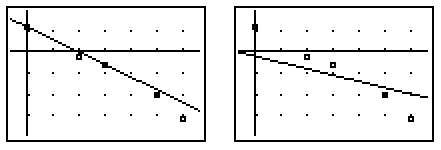
\includegraphics[width=0.7\linewidth]{least_squares}
\end{figure}

Hierdoor kan dus gesteld worden dat door $\beta$\textsubscript{0} en $\beta$\textsubscript{1} te vari\"{e}ren en te kijken welke parametercombinatie voor de curve zal zorgen waarvan de afstand van de datapunten en die curve het laagst is, bepaald kan worden welke waarden voor  $\beta$\textsubscript{0} en $\beta$\textsubscript{1} optimaal zijn.

De accuraatheid van een curve kan dus weergegeven aan de hand van formule 2.2.

\begin{equation}
Error = \sum(actual\;output - predicted\;output)^2
\end{equation}

Nu rijst de vraag hoe de parameters zodanig kunnen evolueren zodat ze de kleinst mogelijke foutmarge benaderen. Dit wordt gerealiseerd aan de hand van gradient descent een uitgebreide uitleg van gradient descent komt aan bod bij het bespreken van de LSTM techniek maar het komt er op neer dat gradient descent er zal voor zorgen dat de optimale parameters zo nauwkeurig mogelijk bepaald zullen kunnen met een zo laag gebruik van middelen.

%, dit wordt grafisch weergegeven op figuur 2.2 waarbij J($\theta_0\theta_1$) de foutmarge weergeeft en $\theta_0$ en $\theta_1$ de variabelen weergeven. Gradient descent zal er dan voor zorgen dat men in een dal zal terechtkomen en dus de parameters voor de laagste foutmarge bepaald kunnen worden. De stapgrootte waarmee afgedaald wordt is bij het minimaliseren van de foutmarge zeer belangrijk. Een grotere stapgrootte zullen de optimale parameters snel bepaald kunnen worden maar zullen ze niet nauwkeurig zijn. Terwijl een kleinere stapgrootte voor een heel hoge uitvoeringstijd zal kunnen zorgen maar wel zeer nauwkeurig zal zijn en je effectief in het laagste punt van het grafische dal zal terechtkomen. Gradient descent zal de stapgrootte verkleinen naargelang de foutmarge kleiner wordt en de optimale foutmarge dus op een nauwkeurige manier bepaald zal kunnen worden zonder relatief veel middelen te benutten.



\begin{table}[ht]
    \caption{Voorbeelddata voor lineaire regressie~\autocite{Pant2019}}
    \centering
    \begin{tabular}{|c|c|} 
        \hline     
        Living area (feet\textsuperscript{2}) & Price (1000\$) \\ [0.5ex] 
        \hline\hline
        2104 & 400 \\  [0.3ex]
        \hline
        1600 & 330 \\ [0.3ex]
        \hline
        2400 & 369 \\ [0.3ex]
        \hline
        1416 & 232 \\ [0.3ex]
        \hline
        3000 & 540 \\ [0.3ex]
        \hline
    \end{tabular}
    \label{Tab:Tcr}
\end{table}

\begin{figure}[!h]
    \centering
    \caption{Grafische weergaven voorbeelddata voor lineaire regressie~\autocite{Pant2019}}
    \label{fig:ExampleDataLinearRegressionGraph}
    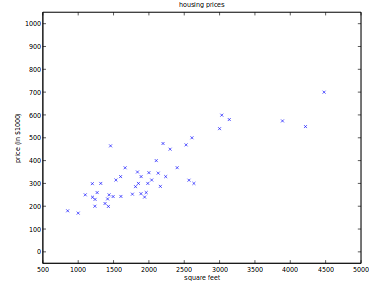
\includegraphics[width=0.7\linewidth]{ExampleDataLinearRegressionGraph}
\end{figure}

%\begin{figure}[!h]
%    \centering
%    \caption{Grafische weergave van gradient descent}
%    \label{fig:GradientDescend3D}
%    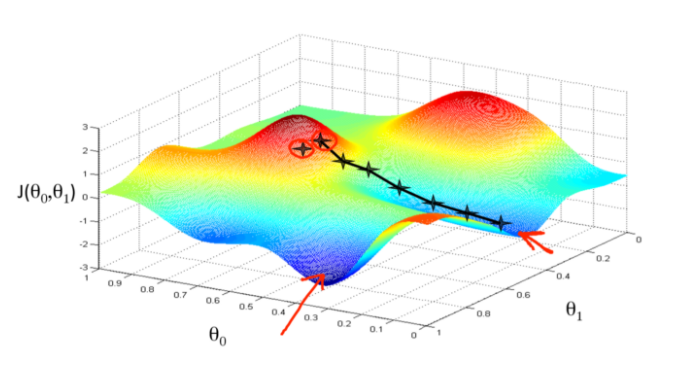
\includegraphics[width=0.7\linewidth]{GradientDescend3D}
%\end{figure}

\subsection{\IfLanguageName{dutch}{Polynomiale Regressie}{Polynomial Regression}}

Soms zal de foutmarge bij data hoog blijven bij lineaire regressie ook al is er een verband zichtbaar, dit verband zal dan waarschijnlijk niet te vatten vallen onder een gewone rechte. In zo'n geval kan polynomiale regressie hulp bieden, dit zal een complexere functie aan de data proberen fitten. Formule 2.3 is dan formule van een $2^{de}$ graadsfunctie 

\begin{equation}
y = \beta_0 + \beta_1 x_1  + \beta_2 x_2^2 
\end{equation}

Dit zorgt ervoor dat de algemene formule herleid wordt naar de formule 2.4 indien we een polynomiale vergelijken wensen toe te passen bij de regressieanalyse.

\begin{equation}
y = \beta_0 + \beta_1 x  + \beta_2 x^2 + ... + \beta_m x^m + residual\;error
\end{equation}

Ook bij polynomiale regressie wordt gebruik gemaakt van gradient descent om de minimale kost te berekenen aangezien dit in principe een uitbreiding is op lineaire regressie. 

Dus polynomiale regressie zal de beste gemiddelde inschatting kunnen maken van de relatie tussen de afhankelijke en onafhankelijke variabelen. De curve die gefit moet worden zal zeer complexere vormen dan een simpele rechte kunnen aannemen en meer dan enkel lineaire verbanden kunnen deduceren uit de data. Het grootste nadeel van polynomiale regressie is dat enkele uitschieters de resultaten sterk kunnen be\"{i}nvloeden terwijl er bij lineaire regressie meer validatietechnieken beschikbaar zijn voor het achterhalen van uitschieters \autocite{Pant2019}. 



\subsection{\IfLanguageName{dutch}{Logistische Regressie}{Logistic Regression}}

Logistische regressie is gelijkaardig aan lineaire regressie maar in tegenstelling tot lineaire regressie zal dit voornamelijk gebruikt worden voor classificatieproblemen, waarbij dus geen continue waarden dienen voorspeld te worden maar nominale waarden. Onder zijn meest simpele vorm zal dit type algoritme nuttig zijn bij het voorspellen van binaire waarden bijvoorbeeld indien men al dan niet aan een aandoening zal lijden. Dit wordt benoemd als binaire logistische regressie. Wanneer er 3 of meer categori\"{e}n die dienen voorspeld te worden waarvan de ene niet duidelijk hoger of lager is dan de andere zoals bijvoorbeeld type huisdier wordt dit benoemd als multinomial logistic regression. Indien er wel een logische ordening in zit zoals een aantal sterren op een filmbeoordeling wordt dit benoemd als ordinale logistische regressie.
Aangezien in deze paper enkel continue waarden voorspeld zullen worden, zal hier niet dieper op in gegaan worden~\autocite{Swaminathan2018}.

\subsection{\IfLanguageName{dutch}{Meervoudige lineaire regressie}{Multiple Linear Regression}}

Indien er meerdere onafhankelijke variabelen beschikbaar zijn die een lineaire invloed zouden hebben op de afhankelijke variabele kunnen deze ook in rekening gebracht worden. Dit model zal dan opgesteld worden aan de hand van meervoudige lineaire regressie ofwel multiple linear regression. Formule 2.5 geeft weer hoe de onafhankelijke waarden bij meervoudige lineaire regressie berekend zullen worden.

\begin{equation}
y_i = \beta_0 + \beta_1 {x_i}_1 + \beta_2 {x_i}_2 + ... + \beta_n {x_i}_n + \epsilon_i
\end{equation}

Net zoals bij enkelvoudige lineaire regressie zal $y\textsubscript{i}$ de afhankelijke variabele weergeven en $\beta$\textsubscript{0} het intercept. Het verschil zit hem in de termen die volgen want aangezien er rekening gehouden wordt met meerdere onafhankelijke variabelen, zullen ook deze verwerkt worden in de formule door middel van een waarde te voorzien voor elke onafhankelijke variabele weergegeven door $X\textsubscript{i}$ met bijhorend intercept weergegeven door $\beta$. De $n$ in de formule geeft dan het aantal onafhankelijke variabelen weer. De $\epsilon$\textsubscript{i} zal ook in dit geval een factor zijn die rekening zal houden met de meetfouten~\autocite{Kenton2020}.

\subsection{\IfLanguageName{dutch}{Toepassing}{}}

Deze regressietechnieken zullen dienen als basis voor andere meer uitgebreide technieken zoals ARIMA maar de verbanden die ze weergeven zijn te eenvoudig om effectief te gebruiken voor het opbouwen van modellen om aan extrapolatie te doen.~\autocite{Sinha2019} Daarom zullen de klassieke regressiemethodes niet toegepast worden bij deze bachelorproef. 

%\subsection{\IfLanguageName{dutch}{Meervoudige polynomiale regressie}{Multiple Polynomial Regression}}

\section{\IfLanguageName{dutch}{ARIMA}{Prediction Techniques}}
\label{sec: Theoretische toelichting over ARIMA}

ARIMA is een modeleringstechniek die voorspellingen maakt op basis va, stationaire en gedifferenti\"{e}erde data. Daarom worden deze begrippen eerst toegelicht alvorens de techniek zelf te bespreken. 

\subsection{\IfLanguageName{dutch}{Stationariteit}{Stationarity}}

Een stationaire tijdreeks is een tijdreeks waarvan de eigenschappen niet afhankelijk zijn van het tijdstip waarop de reeks wordt geobserveerd~\autocite{Hyndman2018}. Indien er een duidelijke trend dus een algemene stijging of daling aanwezig is zal de tijdreeks niet stationair zijn. Ook wanneer er een seizoensverband aanwezig is die lijkt op een sinus of cosinusfunctie wordt de data als niet stationair beschouwd. Wanneer er echter een cyclisch verband aanwezig is kan er een speciaal type ARIMA model gebruikt worden dat rekening zal houden met deze seizoenscomponent genaamd SARIMA deze zal zodadelijk toegelicht worden.
In figuur 2.3 zijn enkele voorbeeldtijdreeksen zichtbaar dit toont aan dat het niet zo evident is om te bepalen welke tijdreeks stationair is.

\begin{figure}[!h]
    \centering
    \caption{Voorbeeldtijdreeksen~\autocite{Hyndman2018}}
    \label{fig:stationarity}
    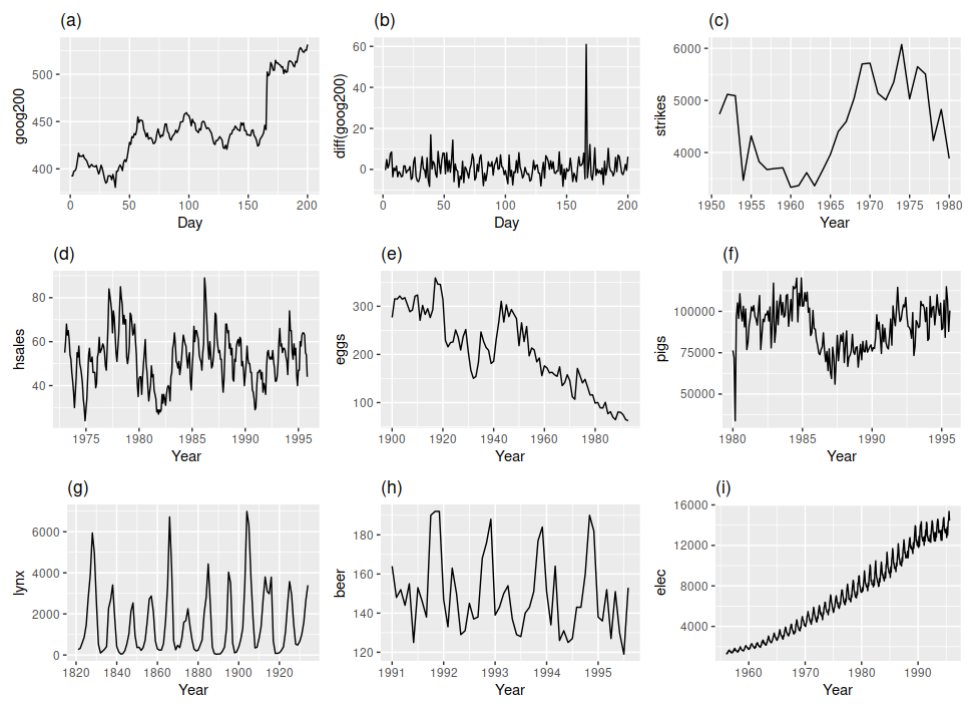
\includegraphics[width=0.7\linewidth]{stationarity}
\end{figure}

De cijfers in de figuur omschrijven de volgende data:

\begin{enumerate}[label=(\,\alph*)\,]
    \item De aandeelkoersen van Google voor 200 opeenvolgende dagen
    \item De dagelijkse veranderingen in de aandeelkoersen van Google voor 200 opeenvolgende dagen
    \item Het jaarlijkse aantal stakingen in de Verenigde Staten
    \item Maandelijkse verkoop van nieuwe gezinswoningen in de Verenigde Staten
    \item Jaarlijkse prijs van een dozijn eieren in de Verenigde Staten (rekening houdend met inflatie)
    \item Maandelijks aantal varkens die geslacht worden in Victoria, Australi\"{e}
    \item Jaarlijks aantal lynxen die opgesloten worden in het McKenzie River district van noordwest Canada
    \item Maandelijkse Australische bierproductie
    \item Maandelijkse Australische elektriciteitsproductie
\end{enumerate}

\subsection{\IfLanguageName{dutch}{Seizoenseffect}{Seasonality}}

Bij de figuren (d), (h) en (i) is er een duidelijk seizoenseffect zichtbaar. Er vallen duidelijke trends waar te nemen op figuren (a), (c), (e), (f) en (i). Ook in figuur (g) lijkt er een duidelijk seizoenseffect te zijn, maar deze veranderingen zijn aperiodisch dus op lange termijn valt dit niet te voorspellen aldus is deze tijdreeks stationair.


\subsection{\IfLanguageName{dutch}{Differentiatie}{Differencing}}

Aan de hand van deze grafieken kan ook een ander begrip toegelicht worden dat een belangrijk gegeven is bij het opstellen van een ARIMA model namelijk differentiatie. Zo wordt op figuur (a) de aandeelkoers van google weergegeven voor 200 opeenvolgende dagen, maar hier is een duidelijk stijgende trend zichtbaar. Hierdoor kan de data niet op deze manier ge\"{i}nterpreteerd worden door een ARIMA model. Maar we kunnen de data op een andere manier voorstellen namelijk door de koerswissellingen zoals weergegeven wordt op figuur (b) waardoor er geen trend meer aanwezig zal zijn en nog steeds geen zichtbare seizoensgebondenheid aanwezig is. 

\subsubsection{\IfLanguageName{dutch}{Random walk differentiatie}{Random walk model}}
Bij random walk differencing wordt de data gediffernti\"{e}erd door het verschil te nemen tussen een tijdstap en de tijdstap die ervoor komt. Dit zal de evolutie van de tijdreeks weergeven en aangeven hoeveel een waarde precies verschilt van de tijdstap ervoor. Deze differentiatie kan uitgedrukt worden als

\begin{equation}
y_t^\prime = y_t - y_{t-1}.
\end{equation}

De gedifferenti\"{e}erde reeks zal 1 waarde minder hebben dan de originele serie omdat er geen waarde voor de eerste $y_1^\prime$ komt om deze te differenti\"{e}ren.
 
Wanneer de gedifferentiëerde reeks ruis is kan het model uitgedrukt worden als 
 
\begin{equation}
y_t - y_{t-1} = \epsilon_t,
\end{equation}

Hierbij zal $epsilon_t$ de ruis weergeven. Door deze formule te hervormen bekomen we het ''random walk model".

Deze modellen worden vaak gebruikt voor niet-stationaire data, voornamelijk bij financi\"{e}le en economische toepassingen.

De voorspellingen van dit model zijn gelijk aan dit de laatste observatie.

\subsubsection{\IfLanguageName{dutch}{Tweedegraadsdifferentiatie}{Second order differencing}}

In sommige gevallen zal gedifferencieerde data nog steeds niet stationair zijn dan is het eventueel mogelijk om de gedifferenti\"{e}erde nogmaals te differenti\"{e}ren. Dit kan als volgt geformuleerd worden.

\begin{equation}
\begin{aligned}
y_t^n {} & = y^\prime_t - y^\prime_{t-1}  \\
& = (y_t - y_{t-1}) - (y_{t-1} - y_{t-2})\\
& = y_t - 2y_{t-1} - y_{t-1}
\end{aligned}
\end{equation}

Op deze manier kan een verandering in de veranderingen gedetecteerd worden. Uiteraard zou men nog een stap verder kunnen gaan maar dit blijkt in praktijk zo goed als nooit nodig te zijn.

\subsubsection{\IfLanguageName{dutch}{Seizoensdifferentiatie}{Seasonal differencing}}
Een laatste manier om data te differenti\"{e}ren is seizoensdifferentiatie. Hierbij zal telkens het verschil genomen worden van een tijdstap en diezelfde tijdstap van de vorige seizoenscyclus. Dit kan als volgt weergegeven worden,

\begin{equation}
y_t^\prime = y_t - y_{t-m}.
\end{equation}

Hier zal $m$ slaan op het aantal observaties in een seizoen. Indien deze data, die seizoensgedifferenci\"{e}erd is, ruis blijkt te zijn dan zou een geschat model voor de originele data kunnen geformuleerd worden als

 \begin{equation}
y_t - y_{t-m} = \epsilon_t,
 \end{equation}

Om seizoensdifferentiaties en gewone differentiaties uit elkaar te houden worden gewone differentiaties ook benoemd als eerste differentiaties. 

Het is mogelijk dat deze verschillende soorten differentiaties gecombineerd moeten worden om tot een stationaire dataset te komen. Een dataset waarbij het waarschijnlijk nodig zal zijn om eerste differentiaties en seizoensdifferentiaties gecombineerd moeten worden is die van de maandelijkse Australische elektriciteitsproductie zichtbaar op figuur 2.3 (i). Aangezien er een seizoenscyclus en een stijgende trend aanwezig is.

\subsection{\IfLanguageName{dutch}{Toeliching ARIMA}{}}

ARIMA is een acroniem gevormd door AutoRegressive Integrated Moving Average wat vrij vertaald kan worden als het autoregressie ge\"{i}ntegreerde voortschrijdend gemiddelde. Deze benaming geeft ook onmiddellijk de sleutelaspecten van dit model weer. 

Zo staat autoregressief voor het modelleren van een volgende stap in een sequentie als een lineaire functie op basis van de voorgaande waarden in deze sequentie.
\\Daarnaast is ARIMA ook een ge\"{i}ntegreerd model wat inhoudt dat niet de cumulatieve waarden gebruikt worden om voorspellingen te maken maar er gekeken wordt naar het verschil tussen die cumulatieve waarden.
\\Ten slotte wordt ook gekeken naar het voortschrijdend gemiddelde in plaats van naar de ruwe data zelf dit zal ervoor zorgen dat extreme waarden veroorzaakt door anomaliteiten geneutraliseerd worden. Hierdoor zal de globale trend beter waarneembaar zijn.

ARIMA modellen zijn theoretisch gezien, de meest algemene klasse van modellen om een tijdreeks te voorspellen die stationair/stationary gemaakt kan worden. 

Elk van deze componenten is geparameteriseerd en kan dus aangepast worden deze parameters worden benoemd als ($p$, $d$ \& $q$)

$p$: Het aantal verlate observaties die worden opgenomen in het model. Deze worden in het Engels benoemd als lag observations of lag order.
\\$d$: Zal bepalen hoeveel keer ruwe observaties van elkaar afgetrokken worden dit kan ook benoemd worden als de mate van differentiatie of the degree of differencing in het Engels.
\\$q$: Deze parameter zal het aantal tijdstappen waarvan het voortschrijdend gemiddelde genomen wordt aangeven. Deze wordt in het Engels benoemd als the order of moving average. 

Een lineair regressiemodel wordt geconstrueerd met data waarbij er een graad van differentiatie is zodat deze stationair is. Dit houdt in dat trend en seizoensstructuren die het regressiemodel op een negatieve manier be\"{i}nvloeden verwijderd worden.

Bij elke parameter kan ook de waarde 0 opgegeven worden zodat dit aspect horende bij die parameter buiten beschouwing gelaten wordt en dit model effectief gebruikt kan worden als gelijk welke combinatie zoals bijvoorbeeld een autoregressief en een ge\"{i}ntegreerd model al dan niet gebruikmakend van het voortschrijdend gemiddelde~\autocite{Brownlee2018}.

$d$ zal dus de differentiatiegraad weergeven wanneer we hier rekening mee houden kunnen we stellen dat de formule voor ARIMA er als volgt uit zal zien~\autocite{Nau2020}:

\begin{equation}
\hat{y_t} = \mu + \phi_1 y_{t-1} + ... + \phi_p y_{t-p} + \theta_1 \epsilon_{t-1} - ... - \theta_q \epsilon_{t-q}
\end{equation}

Om de werking van ARIMA te schetsen zullen kort enkele basisparametercombinaties toegelicht worden.

\subsubsection{ARIMA(1,0,0)}

Dit zal een autoregressief model van de eerste orde zijn ofwel een first-order autoregressive model. Deze parametercombinatie zal gebruikt worden als de reeks stationair en autogecorreleerd is. Dit zou dus voorspeld kunnen worden door de eigen waarde te nemen en deze op te tellen met een constante. De voorspellingsvergelijking zal er als volgt uit zien:

\begin{equation}
\hat{y_t} = \mu + \phi_1 y_{t-1}
\end{equation}

Dit stelt voor dat er regressie uitgevoerd en kan benoemd worden als een ARIMA(1,0,0) model. Wanneer het gemiddelde van $y$ gelijk is aan nul, zal de constante term achterwege gelaten worden. Indien de hellingsco\"{e}fficient $\phi_1$ positief maar minder dan \'{e}\'{e}n is zal het model de waarde van de volgende periode voorspellen als $\phi_1$ keer zo ver van het gemiddelde dan de waarde van deze periode. 

Indien men een autoregressief model van de 2\textsuperscript{de} orde wil voorstellen zal er bij formule (2.12) rechts een $y_{t-2}$ term toegevoegd worden. Wanneer men een model van nog hogere orde wenst voor te stellen dient men analoog termen toe te voegen. Afhankelijk van de tekens en de grootte van de co\"{e}fficienten zal een ARIMA(2,0,0) model een systeem onderschrijven waarvan de gemiddelde omkering sinuso\"{i}daal oscillerend zal zijn, wat te vergelijken valt met de beweging van massa aan een veer die onderhevig is aan willekeurige uitwijkingen.


\subsubsection{ARIMA(0,1,0)}

Deze vorm van ARIMA past de meest simpele vorm van differentiatie toe namelijk ``random walk'', hierbij zal de eerste differentiatie die zonet besproken is in de sectie differentiatie toegepast worden op de data. Door middel van deze differentiatie kan niet-stationaire data omgevormd kunnen worden naar stationaire data indien dit nog steeds niet het geval is kan deze data in een hogere graad gedifferenci\"{e}erd worden. Dit kan weergegeven onder de vorm van deze formule:

\begin{equation}
\hat{y_t} = \mu + y_{t-1}
\end{equation}

Hier zal de constante term $\mu$ de gemiddelde verandering van periode tot periode weergeven dit kan ook benoemd worden als de ``long term drift'' in $y$. Aangezien het enkel een niet-seizoensgebonden verschil en en een constante term omvat wordt het geclassificeerd als een ``ARIMA(0,1,0) model met constante''. Een random walk zonder drift model zou een ARIMA(0,1,0) model zonder constante zijn.


\subsubsection{ARIMA(1,1,0)}

Deze ARIMA configuratie staat voor een gedifferenci\"{e}erd autoregressief model van de eerste graad. Indien de fouten van een random walk model autogecorreleerd zijn is het mogelijk dat dit verholpen kan worden door een vertraging ofwel lag toe te voegen aan de afhankelijke variabele van de voorspellingsvergelijking. Zo zou dus regressie uitgevoerd worden op het eerste verschil van $y$ en zichzelf, vertraagd met 1 tijdstap. Hierbij zal de vergelijking er als volgt uitzien:

\begin{equation}
\hat{y_t} = \mu + y_{t-1} + \phi_1 (y_{t-1} - y_{t-2})
\end{equation}

\subsubsection{ARIMA(0,1,1)}

Hier wordt de laatste parameter van ARIMA voor het eerst aangesproken de $q$. Hierdoor zal er nu gewerkt worden met een voortschrijdend gemiddelde van de data. Dit zal er voor zorgen dat ruis iets meer geneutraliseerd wordt.

\begin{equation}
\hat{y_t} = \mu + y_{t-1} - \theta_1 e_{t-1}
\end{equation}

De constante $\mu$ kan eventueel achterwege gelaten worden, deze zal er voor zorgen dat de voorspelling op lange termijn eerder hellend zal zijn hierbij zal het ook mogelijk zijn om een negatieve co\"{e}fficient toe te laten. Deze constante zorgt er ook voor dat het ARIMA model een SES model wordt. Indien hier niet voor gekozen wordt zal de voorspelling op lange termijn vlak zijn. Zonder constante wordt dit type model benoemd als simple exponential smoothening indien er een constante gebruikt wordt hier growth aan toegevoegd, wat wijst op de stijgende trend op lange termijn waarvan de helling gelijk is aan $\mu$.

\subsubsection{ARIMA(0,2,1) of ARIMA(0,2,2)}

Deze configuraties zonder constante worden ook benoemd als lineaire exponenti\"{e}le afvlakking. Hier zal de 2\textsuperscript{de} afgeleide genomen worden omwille van de waarde voor $d$. 

\begin{equation}
\hat{y_t} = 2y_{t-1} - y_{t-2} - \theta_1 e_{t-1} - \theta_2 e_{t-2}
\end{equation}

De $\theta_1$ en $\theta_2$ zullen staan voor de MA(1) en MA(2) co\"{e}fficienten. Dit zal overeenkomen met Holt's model en in speciale gevallen met Brown's model. het zal gebruik maken van exponenti\"{e}le gewogen voortschrijdende gemiddeldes om het lokale niveau en lokale trend (local level and local trend) te schatten. Voorspellingen op lange termijn zullen naar een rechte lijn toe convergeren wiens helling zal afhangen van de gemiddelde trend naar het einde van de reeks toe. 

\subsubsection{ARIMA(1,1,2)}

Dit wordt benoemd als damped-trend linear exponential smoothing en wordt weergegeven door de formule:

\begin{equation}
\hat{y_t} = y_{t-1} + \phi_1 (y_{t-1} - y_{t-2}) - \theta_1 e_{t-1} - \theta_2 e_{t-2}
\end{equation}

Dit model zal de lokale trend aan het einde van de reeks extrapoleren maar zal afvlakken naar het einde toe. 

Bij het opstellen van een ARIMA mode wordt aangeraden om een van de parameters $p$ of $q$ niet groter te laten worden dan 1 aangezien er een hoge waarschijnlijkheid is dat dit zal leiden tot overfitting of andere fouten.

Een manier om de corelaties en een eventueel vertraagd effect te identificeren tussen de waarden rekening houdend met trend, seasonality en het residu is een ACF ofwel een auto-corelation function~\autocite{Salvi2020}.

Een aanvulling daarop is een PACF ofwel een partial auto-correlation function deze zal eventuele correlaties wanneer de effecten na eerdere vertragingen verwijderd worden (door middel van ACF) weergeven. 

Een goede vuistregel bij het opstellen van een ARIMA model is het verhogen van de $p$ indien er een positieve correlatie is dit houdt in dat de afhankelijke variabele zal stijgen als de onafhankelijke variabele stijgt. Wanneer er een negatieve corelatie is en de onafhankelijke variabele stijgt zal de afhankelijke variabele dalen en in dit geval is het beter om de $q$ te verhogen.

Een stappenplan om ARIMA toe te passen op een dataset zal er als volgt uit zien:

\begin{enumerate}
    \item Plot de data en identificeer ongewone waarden
    \item Transformeer de data om de variantie te stabiliseren indien nodig
    \item Als de data niet stationair is neem eerste differentiaties van de data totdat deze stationair is.
    \item Onderzoek de ACF/PACF en kijk of een ARIMA(p,d,0) of ARIMA(0,d,q) model gebruikt moet worden
    \item Test de modellen uit en gebruik AICc (een scoringstechniek) om het model te verbeteren.
    \item Bekijk de residuen van het gekozen model door ze te plotten samen met de ACF en een portmanteau test van de residuen te doen. Indien deze er niet uitzien als ruis is het aangeraden een nieuw model te proberen
    \item Wanneer de residuen er uitzien als ruis kunnen voorspellingen gemaakt worden   
\end{enumerate}


\subsection{\IfLanguageName{dutch}{Varianten op ARIMA}{Variants of ARIMA}}

\subsubsection{\IfLanguageName{dutch}{SARIMA}{SARIMA}}

In sommige gevallen blijkt er een seizoensgebondenheid aanwezig te zijn in de data. Deze seizoensgebondenheid zal zorgen voor constante fluctuaties.
Deze manier van be\"{i}nvloeden is iets waar bij een gewoon ARIMA model geen rekening mee wordt gehouden. Daarom is er een variant op het ARIMA model genaamd SARIMA waarbij de toegevoegde S zal staan voor de seizoensgebondenheid. Dit zal in rekening gebracht worden door extra parameters toe te voegen. Zo zullen de parameters bij ARIMA $(p,d,q)$ zijn, terwijl de parameters bij SARIMA $(p, d, q)(P, D, Q)m$ zijn, waarbij $m$ zal staan voor het aantal tijdsstappen binnen een seizoenscyclus. Zo zal bij een jaarlijkse cyclus $m$ gelijk zijn aan 12 als de tijdspanne tussen de observaties 1 maand bedraagt. Daarnaast zal de $p$ staan voor autoregressieve seizoensorde ofwel de seasonal autoregressive order, $d$ voor de gedifferenc\"{i}eerde seizoensorde ofwel de seasonal difference order en $q$ voor de seizoensorde van het voortschrijdend gemiddelde ofwel de seasonal moving average order ~\autocite{Brownlee2018a}.

\subsubsection{\IfLanguageName{dutch}{VARMAX}{VARMAX}}
Wanneer er meerdere tijdsreeksen voorspeld moeten worden waarbij er een verband mogelijk zou kunnen zijn tussen de verschillende tijdsreeksen kan de VARMAX techniek gebruikt worden. Hierbij zal de V staan voor vector wat duidt op het interpreteren en voorspellen van vectoren. Dit type model zal dan ook gebruikt worden bij het voorspellen van multivariate of meervoudige tijdreeksen AR wijst andermaal op autoregressief. MA slaat ook weer op het voortschrijdend gemiddelde. De X in VARMAX staat voor de invloed van exogene factoren op de factoren die voorspeld moeten worden. 

\section{\IfLanguageName{dutch}{Long Short Term Memory}{Prediction Techniques}}
\label{subsubsec: Theoretische toelichting van long short term memory netwerken (LSTM)}

Als tweede methode die gebruikt zal worden om tijdreeksen te voorspellen wordt gekozen voor een recurrent neuraal netwerk met gebruik van Long Short Term Memory modellen wat afgekort wordt als LSTM.

Een recurrent neuraal netwerk zal uitgebreid toegelicht worden in de volgende secties maar dit kan kort omschreven worden als een structuur die gebruik maakt van trainingsdata om te ``leren'' en op basis van dit leerproces voorspellingen kunnen maken van nieuwe data. Om dit met een simpel voorbeeld te schetsen zou een neuraal netwerk net zoals wij als mens leren dat er bij veel bewolking kans zal zijn op regen. Om dit te realiseren zullen alle parameters echter numeriek doorgegeven moeten worden aan het neuraal netwerk in dit geval zou een soort van bewolkingsgraad aangewezen zijn. Op basis daarvan zal het neuraal netwerk dan een kans op regen kunnen aangeven. 

Een LSTM is een type recurrent neuraal netwerk dat gebruikt wordt bij sequenti\''{e}le voorspellingsproblemen. Dit betekent dat de volgorde van de data een rol zal spelen en dat bij het voorspellen van een waarde in een reeks rekening zal gehouden worden met een aantal waarden die vlak voor de te voorspellen waarde komen. 


\subsection{\IfLanguageName{dutch}{Theoretische toelichting}{}}
\label{subsec: Theretische toelichting van long short term memory netwerken (LSTM)}

Een neuraal netwerk valt makkelijkst te vergelijken met een menselijk brein. Zo zullen wij bijvoorbeeld het cijfer 1 herkennen aan zijn vormen. Door de verschillende pixels, gebruikt voor het weergeven van ons cijfer 1 als inputwaarden voor een neuraal netwerk te gebruiken en de outputwaarden gelijk te stellen met cijfers 0 tot en met 9 kan het netwerk aangeleerd worden deze cijfers te herkennen. 

Dit gebeurt niet vanzelf maar door een combinatie van eenvoudige rekeneenheden die verbonden zijn en waartussen er verbindingen zijn die beschreven worden met een re\"{e}el getal dat de sterkte van een verbinding aangeeft~\autocite{Lievens2018a}. Zo'n combinatie van eenvoudige rekeneenheden die ook benoemd worden als neuronen wordt net zoals bij het menselijk brein een neuraal netwerk genoemd dit wordt weergegeven op figuur 2.4. 

\begin{figure}
    \centering
    \caption{Voorstelling van een neuron die invoer ontvangt van 3 andere neuronen ~\autocite{Lievens2018a}}
    \label{fig:neuron}
    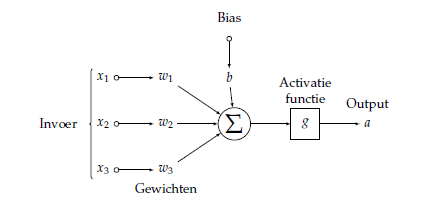
\includegraphics[width=0.7\linewidth]{neuron}
\end{figure}

Zo bevinden zich tussen de input en de outputlaag verschillende lagen die benoemd worden als verborgen lagen. In deze lagen bevinden zich knooppunten (neuronen) waarin waarden worden berekend die een interpretatie geven van de inputwaarden waarmee ze verbonden zijn. Wanneer we dit toepassen op ons voorbeeld zou in een knooppunt bijvoorbeeld kunnen bekeken worden of er in het midden van de te interpreteren pixels een lijn staat. Wanneer dit het geval zou zijn zou er in dit neuron een grote waarde weergegeven worden en zal deze een sterk signaal sturen. Wanneer we voor dit voorbeeld met 1 verborgen laag zouden werken zou het neuron dat een sterk signaal zendt bij het herkennen van een centrale verticale lijn een belangrijke waarde zijn voor het herkennen van een 1 en een 4. De sterke van dit signaal zal dus een grote invloed hebben op de kans dat het resultaat een 1 of een 4 is.
Wanneer we hier dieper op ingaan kunnen we aan elk neuron een formule toewijzen die er zo uitziet:

\begin{equation}
n=w_1 i_1+w_2 i_2
\end{equation}

W staat voor de gewichten, $i$ staat voor de inputwaarde. Stel dat bij dit neuron de bovenste 3 pixels genomen worden en we voor de eenvoud werken met een 3x3 afbeelding, dan zal de formule er als volgt uitzien:

\begin{equation}
n=w_1 i_1+w_2 i_2+ w_3 i_3
\end{equation}

$n$ zal dan staan voor gewogen gemiddelde, door hier een bias aan toe te voegen $b$ net zoals bij lineaire regressie en dit als invoer te gebruiken voor een activatiefunctie $g$ zal de sterkte van het uitvoersignaal bekomen worden. 


Indien een neuron effectief geactiveerd wordt zal bepaald worden door de volgende formule.

\begin{equation}
a = g(n + b)
\end{equation}

Een bias $b$ zal bij een neuraal netwerk zorgt voor een correcte neutrale toestand binnen een neuraal netwerk wanneer alle features nul zijn net zoals bij lineaire regressie.  

Door het gebruik van een activatiefunctie $g$ zal dit netwerk ook meer beginnen lijken op de werking van neuronen zoals ze voorkomen in de natuur. 

Een activatiefunctie zal gebruikt worden om voor non-lineariteit te zorgen binnen het model. Wanneer we de activatiefunctie zouden laten wegvallen zou het volledige neurale netwerk kunnen herleid worden tot \'{e}\'{e}n lineaire functie waardoor er enkel weer lineaire verbanden gelegd kunnen worden. Het toevoegen van een activatiefunctie zal er voor zorgen dat de lineariteit gebroken wordt en er binnenin het netwerk nieuwe, abstracte features gegenereerd kunnen worden die kunnen resulteren in een betere interpretatie van de invoerdata.



\paragraph{Toepassing}
Bij dit voorbeeld zijn we nog steeds op zoek naar een 1 en kennen een hoge waarde toe aan donkere kleuren opdat het model de afbeelding zou kunnen interpreteren. Dit zou betekenen dat $i_1$ en $i_3$ een lage waarde moeten hebben en $i_2$ een hoge waarde. In dit geval zullen de gewichten voor $w_1$ en $w_3$ gelijkgesteld worden aan -1 en het gewicht voor $w_2$ aan 1. Daardoor zal n een hoge waarde krijgen als de centrale pixel zwart is en de buitenste pixels wit. Dit wordt de propagation function genoemd. Om deze waarden om te zetten naar een waarde die interpretabel is doorheen het volledige model wordt het resultaat van de propagation function nog eens gebruikt als invoerwaarde voor een activatiefunctie. In dit geval zou de hyperbolic tangent (tanh) een goede keuze zijn, maar dit hangt af van de toepassing.
Bij dit voorbeeld zou dat signaal dan naar de outputlaag gestuurd worden die op zijn beurt ook weer diezelfde formule toepast maar dan niet met de invoerwaarden maar met de resultaten uit de verborgen laag. Hieruit zal dan een score zou komen die aangeeft hoe waarschijnlijk het is dat de waarden die de pixels weergeven uit de invoerlaag het cijfer vormen dat toegekend is aan dit neuron in de uitvoerlaag. 

Deze toepassing waarbij een cijfer wordt herkend is een voorbeeld van een toepassing van voorwaards gerichte neurale netwerken omdat de data slechts in 1 richting verloopt, een resultaat wordt niet be\"{i}nvloed door voorgaande inputwaarden. Bij recurrente neurale netwerken is dit wel het geval. Hierbij wordt rekening gehouden met de beoordelingen van voorgaande inputwaarden een voorbeeld hiervan is het beoordelen van zinnen de volgorde van de ingevoerde woorden zal een rol spelen. Zo zal `eet ik` ge\"{i}nterpreteerd kunnen worden als een vraag aan de hand van de woordanalyse. Terwijl 'ik eet' zal beoordeeld worden als een statement. 

Dit zal louter gebeuren op basis van de woordvolgorde waarbij connecties tussen verschillende cellen teruglopend kunnen zijn onder elkaar en de vorige inputwaarden dus een invloed zullen hebben op de beoordeling van de volgende inputwaarden~\autocite{Lievens2018a}.

Dit is dus een gelijkaardige werking aan voorwaarts gerichte neurale netwerken maar de signalen verlopen niet allemaal in dezelfde richting binnen het netwerk. Zo kan er een signaal van de 2\textsuperscript{de} verborgen laag teruggestuurd worden naar de 1\textsuperscript{ste} verborgen laag. Op die manier hebben de waarden van vorige iteraties een impact op de volgende resultaten en dit is wat we willen bereiken. 

Een lus van eenzelfde stuk uit het neuraal netwerk die informatie van vorige iteraties doorgeeft aan zichzelf dit wordt weergegeven op Figuur \ref{fig:lstmfig1}.

\begin{figure}[!h]
    \centering
    \caption{Cel in een neuraal netwerk dat gegevens van een andere cel gebruikt om een nieuw signaal uit te sturen~\autocite{Olah2015}}
    \label{fig:lstmfig1}
    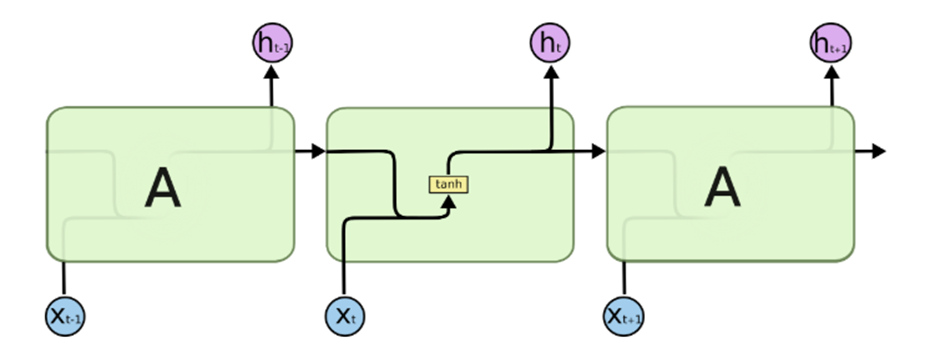
\includegraphics[width=0.7\linewidth]{lstmFig1}
\end{figure}

Om het verloop van een tijdreeks te voorspellen moet ook rekening gehouden worden met het tijdsverloop. Zo zal het verloop van de vorige dagen een invloed hebben op het verloop van de volgende dagen. Dus voor deze toepassing zullen recurrente neurale netwerken gebruikt worden aangezien voorwaarts gerichte neurale netwerken geen rekening houden met de voorgaande inputwaarden. 

Het probleem bij gewone recurrente neurale netwerken is dat deze moeilijk patronen herkennen op lange termijn. Hiervoor biedt de long short term memory variant van recurrente neurale netwerken een oplossing. Dit zorgt ervoor dat enkel de data die bijgehouden moet worden uit vorige iteraties een impact zal hebben op nieuwere resultaten. De werking van een LSTM wordt voorgesteld op figuur \ref{fig:lstmfig2}.

\begin{figure}[!h]
    \centering
    \caption{Gedetaileerdere figuur van een cel uit een neuraal netwerk dat informatie interpreteert uit een andere cel van het neurale netwerk~\autocite{Olah2015}}
    \label{fig:lstmfig2}
    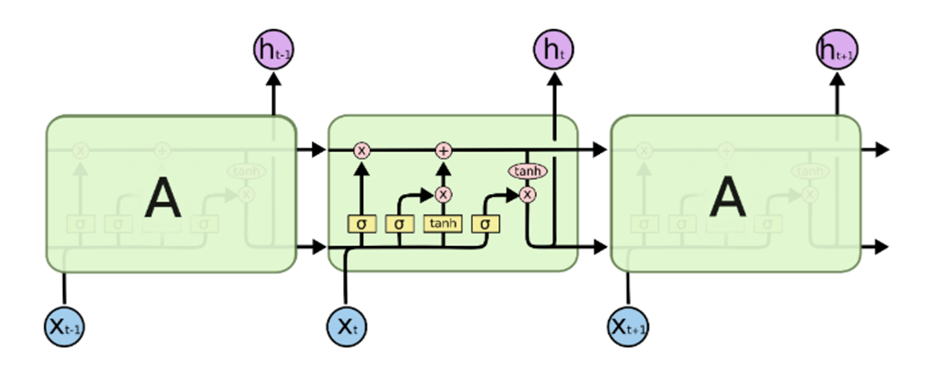
\includegraphics[width=0.7\linewidth]{lstmFig2}
\end{figure}


Dit aan de hand van 4 stappen:
\subparagraph{Stap 1}
Eerst wordt bepaald welke info weggegooid mag worden in de ``forget layer''.
Deze zal een waarde tussen 0 en 1 uitvoeren waarbij een 0 zal betekenen dat deze waarde volledig genegeerd mag worden voor elke component van de cell state en waarbij een 1 zal betekenen dat alles behouden zal moeten worden. 

\begin{figure}
    \centering
    \caption{Grafische weergave van de forget layer binnen het neuron~\autocite{Olah2015}}
    \label{fig:lstmfig3}
    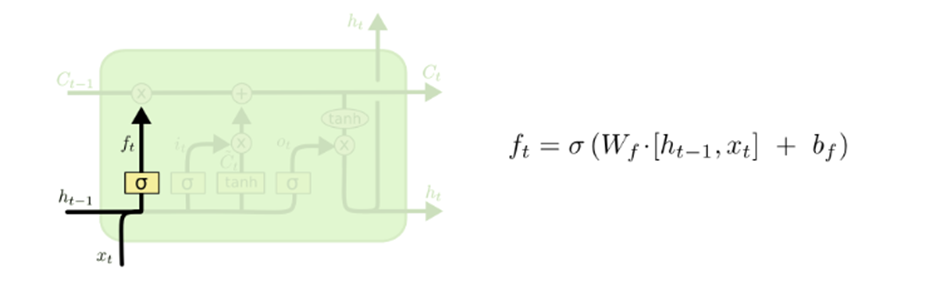
\includegraphics[width=0.7\linewidth]{lstmFig3}
\end{figure}


\subparagraph{Stap 2}
Voor de volgende stap zal in de ``input gate layer'' bepaald worden welke waarden ge\"{u}pdatet moeten worden aan de hand van een sigmo\"{i}de funtie die hier zal resulteren in $i_t$. Daarna zal de vector geconstrueerd worden met de potenti\"{e}le waarden $\tilde{C}_t$.

\begin{figure}
    \centering
    \caption{Grafische weergave van de input gate layer binnen het neuron~\autocite{Olah2015}}
    \label{fig:lstmfig4}
    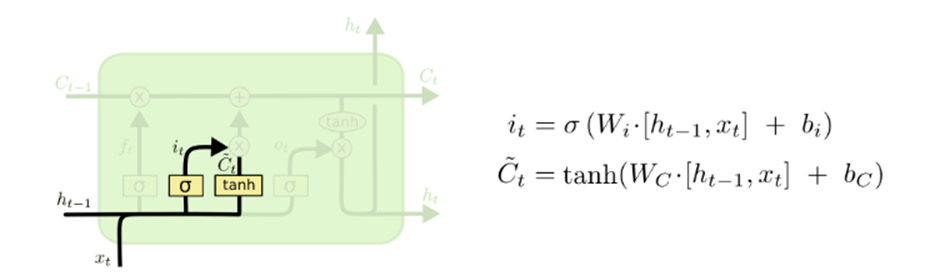
\includegraphics[width=0.7\linewidth]{lstmFig4}
\end{figure}

\subparagraph{Stap 3}
In deze stap zullen we de voorgaande celwaarde vernieuwen. Zo zullen door $C_{t-1}$ te vermenigvuldigen met $f_t$ de overbodige waarden vergeten worden. En door het product van $i_t$ en $C_t$ hierbij op te tellen zullen de achterhaalde waarden ge\"{u}pdatet worden. 

\begin{figure}
    \centering
    \caption{Grafische weergave van het $2^{de}$ deel van de input gateway~\autocite{Olah2015}}
    \label{fig:lstmfig5}
    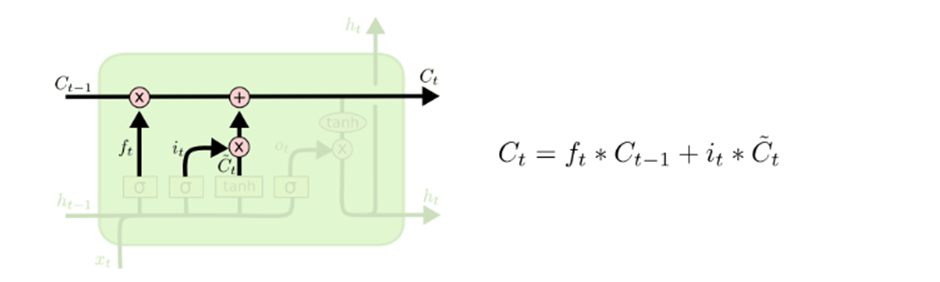
\includegraphics[width=0.7\linewidth]{lstmFig5}
\end{figure}

\subparagraph{Stap 4}
Als laatste zal de uitvoer bepaald worden. Dit is een gefilterde versie van de celtoestand. Die filtering gebeurt aan de hand van een sigmo\"{i}de functie. Het resultaat hiervan wordt dan vermenigvuldigd met de tanh van de celtoestand. Met deze formule verkrijgen we de uitvoerwaarde die de cyclus kan verderzetten.  

\begin{figure}
    \centering
    \caption{Grafische weergave van het onderdeel van de cel waarin de input vermenigvuldigd wordt met de tanh van de celtoestand om de outputwaarde te bekomen~\autocite{Olah2015}}
    \label{fig:lstmfig6}
    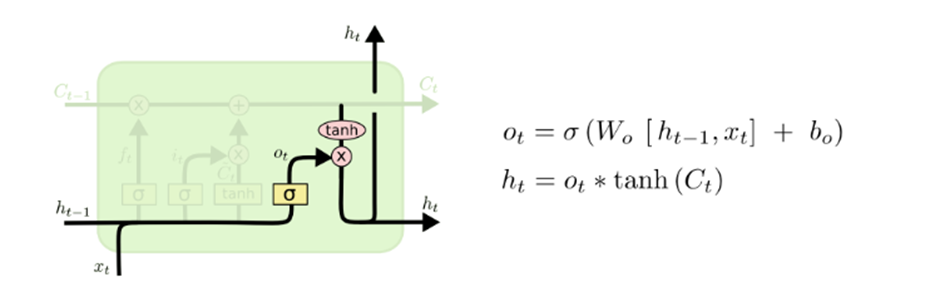
\includegraphics[width=0.7\linewidth]{lstmFig6}
\end{figure}

\subsection{\IfLanguageName{dutch}{Praktische toelichting}{Prediction Techniques}}
\label{subsec: Praktische toelichting van long short term memory netwerken (LSTM)}

Deze praktische toelichting is gebaseerd op het artikel van Jason Brownlee ~\autocite{Brownlee2018b} en zal dienen als basis voor het opstellen van een LSTM netwerk.

\subsubsection{\IfLanguageName{dutch}{Univariate LSTM modellen}{Univariate LSTM models}}

Univariate LSTM models maken voorspellingen voor data waarbij er slechts 1 afhankelijke variabele is.
Hierbij bestaan de problemen uit een reeks observaties. Op basis van vorige waarden in een reeks zal de volgende waarde in diezelfde reeks voorspeld worden. In deze subsectie zullen de voorgestelde modellen toegepast worden op eenstaps univariate tijdreeksen maar deze kunnen makkelijk aangepast worden om gebruikt te worden bij andere soorten tijdreeksen.

\subparagraph{\IfLanguageName{dutch}{Datavoorbereiding}{Data preparation}}
Een tijdreeks zelf bestaat uit een sequentie van waarden zoals hieronder bijvoorbeeld.
\lstset{caption={Originele datasequentie}}
\begin{lstlisting}[language=Python]
[10, 20, 30, 40, 50, 60, 70, 80, 90]
\end{lstlisting}

Om deze waarden te gebruiken voor het trainen van het neuraal netwerk zal deze tijdreeks omgevormd moeten worden naar samples. De dimensies van deze samples zullen bepalen hoeveel inputwaarden en outputwaarden zullen gebruikt worden bij het model. Aangezien we bij dit voorbeeld met eenstapsvoorspellingen werken zal elk sample over 1 outputwaarde beschikken. Bij dit voorbeeld worden 3 inputwaarden genomen. Dit zal als gevolg hebben dat de samples van de gegeven datasequentie er als volgt zullen uitzien.

\lstset{caption={Samples van de gegeven datasequentie}}
\begin{lstlisting}[language=Python]
X,		        y
10, 20, 30		40
20, 30, 40		50
30, 40, 50		60
...
\end{lstlisting}

\paragraph{\IfLanguageName{dutch}{Vanilla LSTM}{Vanilla LSTM}}

Een Vanilla LSTM is een LSTM model dat over \'{e}\'{e}n enkele verborgen laag beschikt en een uitvoerlaag die een voorspelde waarde zal aangeven. In deze verborgen laag zullen zich 50 nodes bevinden. De hoeveelheid te kiezen nodes is afhankelijk van de data. Zo zullen meer nodes de foutmarge verkleinen maar een kleiner aantal nodes zal meer gaan generalizeren, wat het eindresultaat ook zou kunnen verbeteren. Uiteindelijk moet hier een evenwicht in gevonden worden.

Om te bepalen of een signaal binnen een neuron effectief sterk genoeg zal zijn om te activeren en er zelf een te sturen zal de relu activatiefunctie gebruikt worden. Dit is de meest gebruikte activiatiefunctie in neurale netwerken ~\autocite{Liu2017} en heeft als voordeel dat het er weinig complexe wiskunde aan te pas komt bij de berekening waardoor het performant is. Daarnaast convergeert het ook sneller. Door de lineariteit zal de helling niet afvlakken waneer $x$ vergroot. Tenslotte is deze functie ook ijl wat inhoudt dat er altijd iets van activatie is, specifiek bij de relu functie alle waarden onder 0 liggen. Ijlheid komt de effici\"{e}ntie van het model ten goede omdat hierdoor bepaalde neuronen enkel geactiveerd zullen worden bij specifieke prikkels. Zo zou een netwerk voor image recognition een bepaald neuron kunnen hebben dat zal activeren indien er een kattenoor waar te nemen valt, maar het zou niet wenselijk zijn moest dit neuron actief zijn indien er een afbeelding van een gebouw wordt getoond.   

De gewichten van relaties tussen de neuronen in het neuraal netwerk zullen bepaald worden aan de hand van de Adam versie van stochastische gradient descent. Om stochastische gradient descent te defini\"{e}ren zal eerst toegelicht moeten worden wat gradient descent precies inhoudt. Gradient staat voor de afgeleide van de verlies functie en descent betekent afdaling. De combinatie van deze 2 begrippen houdt in dat men zal afdalen tot het laagste punt bereikt wordt~\autocite{Srinivasan2019}.


\begin{figure}
    \centering
    \caption{Parabolische functie}
    \label{fig:parabolicfunction}
    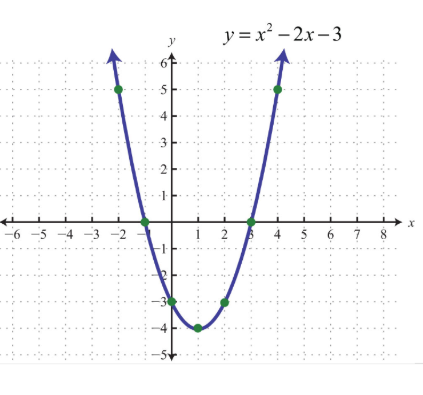
\includegraphics[width=0.7\linewidth]{parabolicfunction}
\end{figure}

We kunnen dit principe makkelijkst voorstellen aan de hand van een parabool. Deze wordt grafisch weergegeven op figuur 2.7. Het minimum van deze parabolische functie wordt bereikt wanneer $x$ een waarde van 1 heeft. 
Als startpunt wordt een willekeurige waarde op de curve genomen waarbij dan nagegaan wordt in welke richting bewogen moet worden om dichter bij het minimum te komen. Wanneer het minimum gezocht wordt zou een stapgrootte gedefinieerd kunnen worden en dan telkens met even grote stappen afgedaald kunnen worden. Wanneer deze stapgrootte bepaald moet worden zou bij een kleine stapgrootte het minimum nauwkeuriger gedefinieerd zijn maar zou dit veel meer berekeningen vergen. Bij een grote stapgrootte zou het minimum snel berekend kunnen worden, maar het zou onnauwkeurig zijn. 

Bij gradient descent wordt deze stapgrootte dynamisch bepaald op basis van het product van de hellingsgraad en de learning rate, een vooraf bepaalde waarde die moet voorkomen dat de stapgrootte te groot wordt. Wanneer de hellingsgraad laag zal zijn betekent dit dat het minimum wordt benaderd en dus kleinere stappen genomen zullen worden om dit zo nauwkeurig mogelijk te bepalen. De kans dat 0 effectief wordt bereikt is zeer klein, daarom stopt het algoritme wanneer een vooraf bepaalde minimale stapgrootte wordt bereikt. Daarnaast kan ook een maximum aantal stappen ingesteld worden waarbij het algoritme stopt. 

Gradient descent kan duidelijk toegelicht worden aan de hand van deze 5 stappen, bij elke stap moet de waarde van de afgeleide opnieuw berekend worden:
\begin{enumerate}
    \item Neem de afgeleide van de verliesfunctie voor elke parameter in deze functie
    \item Kies willekeurige waarden voor deze parameters
    \item Voer de parameterwaarden in in de afgeleiden (in praktijk zal de gradi\"{e}nt numerisch bepaald worden)
    \item Bereken de stapgroottes: Stapgrootte = helling * learning rate 
    \item Bereken de nieuwe parameters: Nieuwe parameter = oude parameter - stapgrootte
\end{enumerate}

Herhaal stappen 3 tot 5 tot het minimum bereikt wordt.

Bij dit voorbeeld zou gewoon de afgeleide van deze parabool kunnen genomen worden om zo tot het minimum te komen, maar bij complexere functies is dit niet mogelijk en biedt gradient descent hiervoor een oplossing.

Bij gebruik van stochastic gradient descent wordt niet telkens alle data gebruikt wanneer de parameters herberekend worden, maar een willekeurige subset uit de dataset om het aantal berekeningen te reduceren wat deze methode performanter maakt zonder al te veel nauwkeurigheid te verliezen~\autocite{Starmer2019}.

Dan rest enkel Adam nog verklaard te worden. Dit is een variant op de klassieke vorm van gradient descent waarbij de learning rate aangepast voor elk gewicht binnen het netwerk en doorheen het trainingsproces.

Deze aanpassingen worden door de auteurs van Adam omschreven als het combineren van 2 andere uitbreidingen op gradient descent namelijk:

Adaptive Gradient Algorithm (AdaGrad) die er voor zorgt dat een per-parameter learning rate die performantie zal verbeteren van de gradi\"{e}nt.  

Root Mean Square Propagation (RMSProp)  deze uitbreiding op gradient descent zorgt voor aanpassingen in de learning rates op basis van de schaal van de laatste gradi\"{e}nten kortom hoe snel deze veranderen~\autocite{Brownlee2017}.


En zal geoptimaliseerd worden op basis van de 'mse' verliesfunctie. 
\captionof{listing}{Datavoorbereiding dataset ijsexpansie}
\label{}
\begin{minted}[
frame=lines,
framesep=2mm,
fontsize=\footnotesize,
linenos,breaklines
]{python}

# univariate lstm voorbeeld
from numpy import array
from keras.models import Sequential
from keras.layers import LSTM
from keras.layers import Dense

# Opslitsen van univariate sequentie in samples
def split_sequence(sequence, n_steps):
X, y = list(), list()
for i in range(len(sequence)):
# vinden van het einde van dit patroon
end_ix = i + n_steps
# nagaan of we ons na de sequentie bevinden
if end_ix > len(sequence)-1:
break
# verwerven van invoer en uitvoerdelen van het patroon
seq_x, seq_y = sequence[i:end_ix], sequence[end_ix]
X.append(seq_x)
y.append(seq_y)
return array(X), array(y)

# Bepalen van de sequentie
raw_seq = [10, 20, 30, 40, 50, 60, 70, 80, 90]

# bepalen van het aantal tijdsstappen
n_steps = 3

# onderverdelen in samples
X, y = split_sequence(raw_seq, n_steps)

# reshape from [samples, timesteps] into [samples, timesteps, features]
n_features = 1
X = X.reshape((X.shape[0], X.shape[1], n_features))

# definieer model
model = Sequential()
model.add(LSTM(50, activation='relu', input_shape=(n_steps, n_features)))
model.add(Dense(1))
model.compile(optimizer='adam', loss='mse')

# fit model
model.fit(X, y, epochs=200, verbose=0)

# demonstreer voorspelling
x_input = array([70, 80, 90])
x_input = x_input.reshape((1, n_steps, n_features))
yhat = model.predict(x_input, verbose=0)
print(yhat)
\end{minted}

\paragraph{\IfLanguageName{dutch}{Stacked LSTM}{Stacked LSTM}}

Een stacked LSTM is een variant op het Vanilla LSTM waarbij er meerdere LSTM lagen na elkaar geplaatst worden. Het toevoegen van een extra laag zal voor een langere uitvoeringstijd zorgen. Het voordeel hiervan is dat hierdoor meerdere onderdelen makkelijker geregistreerd kunnen worden en in verband met elkaar gebracht kunnen worden. Het stapelen van LSTM lagen zal ervoor zorgen dat deze lagen ook onderling uitvoerwaarden zullen uitwisselen die een sequentie van tijdsstappen zal beschrijven en niet gewoon 1 enkele tijdstap~\autocite{Brownlee2017b}.

\begin{figure}
    \centering
    \caption{Een stacked LSTM~\autocite{Brownlee2017b}}
    \label{fig:stacked_lstm}
    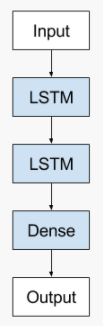
\includegraphics[width=0.15\linewidth]{stacked_lstm}
\end{figure}

\paragraph{\IfLanguageName{dutch}{Bidirectionele LSTM}{Bidirectional LSTM}}

Bidirectionele LSTMs kunnen getrained worden gebruik makend van alle beschikbare invoerinformatie uit het verleden en de toekomst binnen een specifieke tijdspanne. Dit door middel van de toestandsneuronen op te splitsen van een normaal Recurrent Neuraal Netwerk in een deel dat verantwoordelijk is voor de positieve tijdsdirectie en een deel voor de negatieve tijdsdirectie. ~\autocite{Brownlee2017a}

Bidirectionele LSTMs worden voornamelijk gebruikt bij language processing omdat de definitie van een woord afgeleid kan worden uit de context. De begrippen die bepalend zijn voor de definitie kunnen zich zowel voor als achter het woord zelf bevinden dus moet de zin vanuit 2 richtingen geanalyseerd kunnen worden om de definitie te achterhalen.

\begin{figure}
    \centering
    \caption{Weergave van een bidirectioneel LSTM model~\autocite{Colah2015}}
    \label{fig:bidirectional_lstm}
    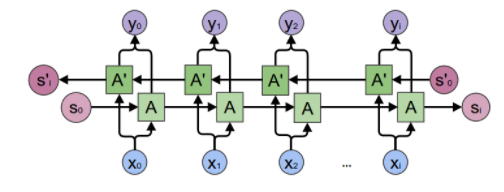
\includegraphics[width=0.7\linewidth]{bidirectional_lstm}
\end{figure}

\paragraph{\IfLanguageName{dutch}{CNN LSTM}{CNN LSTM}}

Een convolutioneel neuraal netwerk ook wel een CNN genoemd wordt voornamelijk gebruikt bij het analyseren van tweedimensionale grafische data. Een CNN is ook sterk in het extraheren en aanleren van features van eendimensionele data. Een CNN model kan ook gecombineerd worden met een LSTM model om een CNN-LSTM te vormen. Hierbij wordt het CNN gebruikt om subreeksen te interpreteren die op zich dan weer zullen ge\"{i}nterpreteerd worden als een reeks door het LSTM model. 

\paragraph{\IfLanguageName{dutch}{ConvLSTM}{ConvLSTM}}

ConvLSTM is ook een soort van CNN-LSTM waarbij het convolutionele deel rechtstreeks is ingebouwd binnen het LSTM gedeelte. Dus ook dit CNN-LSTM werd ontwikkeld voor het interpreteren van tweedimensionale grafische data maar kan aangepast worden voor gebruik bij univariabele tijdreeksvoorspellingen.

\begin{figure}
    \centering
    \caption{\textbf{(a)} Gewone LSTM cell, \textbf{(b)} Weergave van een ConvLSTM~\autocite{Rahman2019}}
    \label{fig:ConvLSTM}
    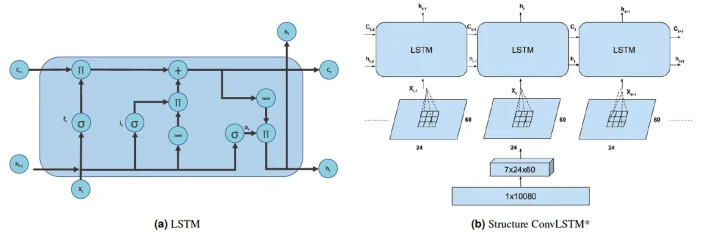
\includegraphics[width=0.7\linewidth]{ConvLSTM}
\end{figure}


\subsubsection{\IfLanguageName{dutch}{Multivariabele LSTM modellen}{Multivariate LSTM models}}

Bij multivariabele tijdreeksen zullen er in tegenstelling tot univariabele tijdsreeksen wel meerdere observaties zijn per tijdseenheid. Deze worden dan nog eens onderverdeeld in multiple input series en multiple parallel series. 

\paragraph{\IfLanguageName{dutch}{Meerdere invoerreeksen}{Multiple Input Series}}

Bij de variant met meerdere invoerreeksen zullen er meerdere invoerwaarden zijn voor elk tijdstip. Hierbij zal slechts voor 1 van de invoerreeksen een voorspelling gemaakt worden. 

\paragraph{\IfLanguageName{dutch}{Meerdere parallelle reeksen}{Multiple Parallel Series.}}
Bij de LSTM variant waarbij er meerdere parallelle reeksen zijn zullen er meerdere invoerwaarden zijn voor elk tijdstip. Hier zal er voor elke reeks een waarde voorspeld worden.


\subsubsection{\IfLanguageName{dutch}{Multi-Step LSTM modellen}{Multi-Step LSTM models}}

Tot nu toe werden enkel maar one-step LSTM modellen toegelicht waarbij de invoerreeks slechts zal resulteren in 1 uitvoerwaarde. Bij multi-step LSTM modellen zal er meer dan 1 uitvoerwaarde voorspeld worden.

\paragraph{\IfLanguageName{dutch}{Vector output model}{Vector output model}}

Bij dit type multi-step LSTM model zal de uitvoer onder de vorm van een vector weergegeven worden die de resultaten van de volgende tijdstappen zal weergeven en niet enkel van de volgende tijdstap. 

\paragraph{\IfLanguageName{dutch}{Encoder-Decoder Model}{Encoder-Decoder Model}}


Dit model is ontwikkeld om sequenties met variabele uitvoer te voorspellen~\autocite{Brownlee2017a}. Het is ook ontworpen om problemen waarbij er zowel invoer-als uitvoersequenties zijn te behandelen. Deze problemen worden ook wel benoemd als sequence-to-sequence of seq2seq-problemen. Deze techniek wordt voornamelijk gebruikt bij vertalingstoepassingen maar kan ook toegepast worden op tijdreeksen. 
Het model bestaat uit 2 hoofdonderdelen de encoder en de decoder. 

De encoder is verantwoordelijk voor het lezen en interpreteren van de invoerreeks. De encoder zal dan een vector met een vaste lengte uitvoeren die een interpretatie zal geven van de invoerreeks. Normaal zal de encoder een Vanilla LSTM model zijn, maar er kan even goed een stacked, bidirectioneel of CNN model gebruikt worden.

De decoder zal de uitvoer van de encoder dan gebruiken als invoer. Die zal dan voor elke tijdsstap een uitvoerwaarde zal geven. Deze uitvoer zal dan nog eens ge\"{i}nterpreteerd worden door een verborgen laag alvorens dit volledig model de multi-step uitvoerreeks zal teruggeven.

\begin{figure}
    \centering
    \caption{Encoder-Decoder Model~\autocite{Brownlee2017a}}
    \label{fig:encoder_decoder_lstm}
    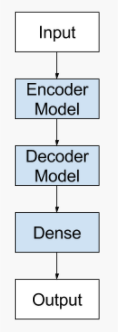
\includegraphics[width=0.15\linewidth]{encoder_decoder_lstm}
\end{figure}


\subsubsection{\IfLanguageName{dutch}{Multivariate Multi-Step LSTM Models LSTM modellen}{Multivariate Multi-Step LSTM Models LSTM models}}

\paragraph{\IfLanguageName{dutch}{Multiple input Multi-Step Output}{Multiple input Multi-Step Output}}

Wanneer men over een dataset beschikt met meerdere invoerparameters maar slechts 1 enkele parameter voor meerdere tijdsstappen dient te voorspellen spreekt men over multiple input multi-step output.

\paragraph{\IfLanguageName{dutch}{Multiple Parallel Input and Multi-Step Output}{Multiple Parallel Input and Multi-Step Output}}

Wanneer de dataset waarvan een voorspelling gemaakt moet worden meerdere invoerparameters heeft maar er  ook meerdere voorspeld moeten worden zal dit benoemd worden als een multiple parallel input and multi-step output LSTM.

\section{\IfLanguageName{dutch}{Prophet}{}}

Prophet is een procedure om tijdreeksen te voorspellen ontwikkeld door Facebook.~\autocite{Prophet2020} Deze procedure baseert zich op een additief model waar niet-lineaire trends gefit worden aan jaarlijkse, wekelijkse en dagelijkse seizoensgebondenheid hierbij zal ook rekening gehouden worden met zogenaamde ``holiday effects'', fluctuaties in de data die veroorzaakt worden door vakantieperiodes. Deze techniek zal best werken met tijdreeksen die een sterk seizoensgebonden effect hebben en waarvan ook meerdere seizoenen aan historische data beschikbaar zal zijn. Daarnaast houdt Prophet ook rekening met ontbrekende data, verschuivingen in de trend en zal het ook rekening houden met uitschieters. 

Het is eenvoudig om te gebruiken maar er zijn ook optimalisaties mogelijk indien men het model wil finetunen. Prophet is zowel beschikbaar in R als in Python



\section{\IfLanguageName{dutch}{Validatietechnieken}{}}

Om de kwaliteit van de modellen te beoordelen zal er telkens een deel van de dataset achtergehouden worden die niet zal gebruikt worden bij het opstellen van het model. Deze achtergehouden dataset wordt de testset genoemd. In het geval van een tijdreeks zullen dit altijd de laatste waarden zijn. Het model zal dan trachten deze laatste waarden te voorspellen waarna de voorspelde waarden vergeleken zullen worden met de waarden van de testset. Op basis hiervan kunnen we achterhalen hoe groot de fout is bij elk model, het model met de laagste fout zal dan de meest accurate voorspelling maken. 
In deze sectie zullen enkele verschillende methodes om de fout te berekenen toegelicht worden ~\autocite{Hyndman2018}.

\subsection{\IfLanguageName{dutch}{Foutmaten}{}}

\subsubsection{\IfLanguageName{dutch}{MAE}{}}
MAE staat voor mean absolute error. Deze zal berekend worden door het verschil te nemen tussen elke voorspelde tijdstap en de verwachte waarde voor deze tijdstap, hier de absolute waarde van te nemen en dan het gemiddelde te nemen van al deze absolute waarden. De formule voor de gemiddelde absolute fout wordt hieronder weergegeven.

\begin{equation}
MAE = \frac{\sum_{i=1}^{n} |y_i - \hat{y_i}|}{n}
\end{equation}

Dit is de meest eenvoudige foutmaat en wordt vaak gebruikt al moet er echter mee rekening gehouden worden dat deze fout eenheidsgebonden is en kan deze niet gebruikt worden om tijdreeksen te vergelijken die gebruik maken van andere eenheden. Dit heeft wel als voordeel dat deze fout makkelijk te interpreteren valt. Zo zou bijvoorbeeld een fout van 1 bij een tijdreeks over temperatuur in graden Celsius betekenen dat de gemiddelde fout bij het voorspellen van de temperatuur 1 graad Celsius is bij dat model.

\subsubsection{\IfLanguageName{dutch}{RMSE}{}}

RMSE staat voor root mean squared error. Deze wordt berekend door het verschil te nemen tussen tussen elke voorspelde tijdstap en de verwachte waarde bij deze tijdstap, dit te kwadrateren, het gemiddelde te nemen van deze kwadraten en dan de vierkantswortel te nemen van dit gemiddelde.
Dit kan ook als volgt geformuleerd worden:

\begin{equation}
RMSE = \sqrt{\frac{\sum_{i=1}^{n} (y_i - \hat{y_i})^2}{n}}
\end{equation}

Ook bij RMSE zal de eenheid gelijk blijven. Het verschil met MAE is echter dat een groot verschil tussen de voorspelde en effectieve waarde zwaarder zal doorwegen bij RMSE doordat deze eerst gekwadrateerd worden voordat het gemiddelde genomen wordt~\autocite{Kampakis2020}.

\subsubsection{\IfLanguageName{dutch}{MAPE \& RMSPE}{}}

MAPE staat voor mean absolute percentage error en RMSPE voor root mean square percentage error. Dit zijn procentuele fouten, dit type fout kan vergeleken worden tussen tijdreeksen met een verschillende eenheid. Dit zijn variaties op respectievelijk MAE en RMSE maar waarbij deler toegevoegd wordt bij het berekenen van het verschil tussen de voorspelde en de effectieve waarde. De formules van deze fouten worden hieronder weergegeven.

\begin{equation}
MAPE = \frac{\sum_{i=1}^{n} |\frac{y_i - \hat{y_i}}{y_i}|}{n}
\end{equation}

\begin{equation}
RMSPE = \sqrt{\frac{\sum_{i=1}^{n} (\frac{y_i - \hat{y_i}}{y_i})^2}{n}}
\end{equation}

\subsection{\IfLanguageName{dutch}{Cross-validation}{}}

Om een tijdreeks nog beter te benutten kan ook cross-validation gebruikt worden. Hierbij zal dezelfde tijdreeks meerdere malen gebruikt worden om het model te trainen, maar zal deze telkens uitgebreid worden zoals zichtbaar in figuur 2.17. De accuraatheid van het model zal dan bepaald worden door de het gemiddelde te nemen van de accuraatheid voor elke opgestelde testset. Er moet echter rekening mee gehouden worden dat deze nieuwe training en testsets altijd nieuwe observaties moeten bevatten en de observaties van de trainingsset altijd moeten voorkomen voor deze van de bijhorende testset~\autocite{Shrivastava2020}.

\begin{figure}
    \centering
    \caption{Grafische weergave van de structuur van een cross-validation tijdreeks~\autocite{Hyndman2018} waarbij 1 tijdreeks zal opgedeeld worden in 20 train- en testreeksen}
    \label{fig:cross_validation_ts}
    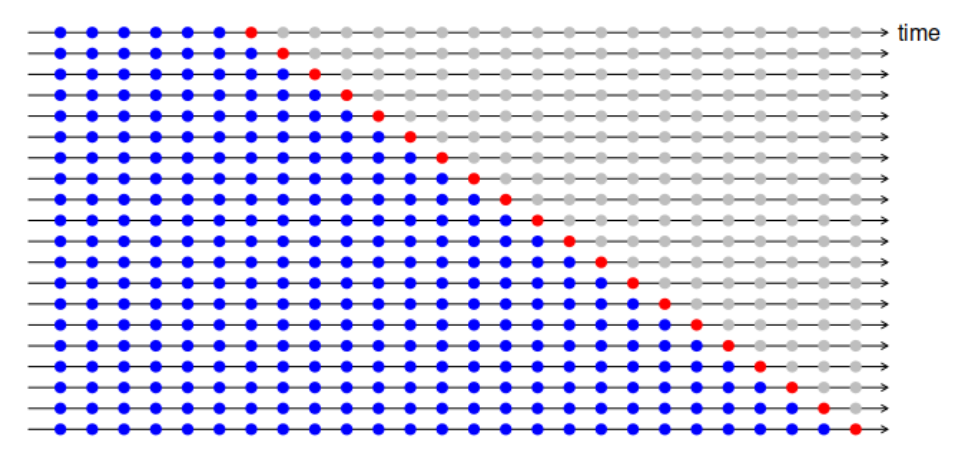
\includegraphics[width=0.9\linewidth]{cross_validation_ts}
\end{figure}


